%----------------------------------------
\begin{frame}
  \frametitle{Part 4}

{\Large\bf Worked examples}

\vspace{0.5cm}

{\large 1. A recent analysis}

\vspace{0.25cm}

{\small A lock-free priority queue, August 2026}

\end{frame}

%----------------------------------------
\begin{frame}[fragile]
  \frametitle{The queue} \small

\begin{block}{The problem}\small
A message queue built on a mutex cannot be used from an interrupt handler, because
a mutex cannot be taken there.
\end{block}

\vspace{0.15cm}

So: replace the mutex with compare-and-swap.

\vspace{0.15cm}

An array of \tool{depth} {\bf slots}. Each holds one message and an atomic word
giving its state --- all \ipromela{FREE} to begin with:

\vspace{0.25cm}

{\centering
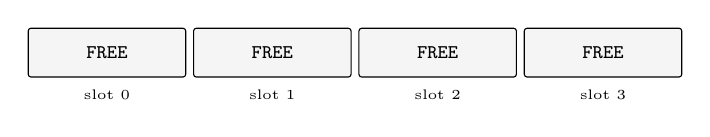
\begin{tikzpicture}
  \foreach \i in {0,1,2,3} {
    \draw[fill=black!4, rounded corners=1pt] (\i*2.1,0) rectangle (\i*2.1+2.0,0.62);
    \node[font=\scriptsize\ttfamily] at (\i*2.1+1.0,0.31) {FREE};
    \node[font=\tiny] at (\i*2.1+1.0,-0.22) {slot \i};
  }
\end{tikzpicture}\par}

\vspace{0.3cm}

{\centering\small
\ipromela{FREE} $\to$ \ipromela{WRITING} $\to$ \ipromela{READY} $\to$
\ipromela{READING} $\to$ \ipromela{FREE}\par}

\vspace{0.25cm}

A producer takes a slot by winning the CAS \ipromela{FREE}$\to$\ipromela{WRITING};
a consumer takes it by winning the CAS \ipromela{READY}$\to$\ipromela{READING}. {\bf Winning
the CAS is what confers ownership} --- two consumers may pick the same slot, only
one wins, so nothing is delivered twice.

\end{frame}

%----------------------------------------
\begin{frame}[fragile]
  \frametitle{And one counter, purely for speed} \small

Scanning the whole array every time, just to see whether there is an element, is
costly --- and it is asked every dispatch cycle.

\pause
\vspace{0.35cm}

\begin{block}{The optimization: \tool{available}}\small
A counter, so a consumer can skip the scan when there are likely no elements.

\vspace{0.15cm}

The count now lives in {\bf two places} --- the counter, and implicitly the slots
themselves. They need not match exactly: the counter is only a hint, and whoever
passes it still runs the real scan. What matters is {\em which way} it is allowed
to be wrong.

\vspace{0.15cm}

It is also public: \tool{getMessagesAvailable()} is downlinked as telemetry.
\end{block}

\end{frame}

%----------------------------------------
\begin{frame}[fragile]
  \frametitle{\tool{send} and \tool{receive}, as written} \small

\begin{lstlisting}[style=shell]
send(m):
    slot = claimFreeSlot()               # CAS FREE -> WRITING
    write(slot, m)
    publish(slot)                        # CAS WRITING -> READY
    available += 1                       # credit it AFTER publishing

receive():
    repeat, at most MAX_RETRY_PASSES times:   # a pass = peek, scan, claim
        if available == 0:      continue      # 1. peek: skip the scan
        slot = selectBestReady()              # 2. scan: claims nothing
        if slot == none:        continue
        if CAS(slot, READY -> READING):       # 3. claim: fails if another
            available -= 1                    #    consumer got there first
            m = read(slot)
            release(slot)                     # CAS READING -> FREE
            return m
        # lost the claim -- yield and try again
    return EMPTY                              # all passes used up
\end{lstlisting}

\pause

No mutex means nothing to sleep on: a blocking caller {\bf polls} the counter, not
the array.

\pause

Only the third step commits to anything: the decrement is authorized by {\bf
winning that CAS}. Two consumers winning on {\em different} slots have both earned
one.

\end{frame}

%----------------------------------------
\begin{frame}[fragile]
  \frametitle{The model --- the producer} \small

Claude Code flagged an issue. I then asked it to generate a \promelaname{} model
to illustrate it.

\begin{lstlisting}[language=promela]
/* FREE=0, WRITING=1, READY=2, READING=3 */
byte slot[2] = FREE;              /* each slot's state */
int  avail = 0;                   /* signed: underflow shows as -1 */
active [2] proctype Producer() {
  int myslot;                     /* the slot this producer claimed */
  do
  :: atomic {                     /* the claim CAS */
       if
       :: (slot[0] == FREE) -> slot[0] = WRITING; myslot = 0
       :: (slot[1] == FREE) -> slot[1] = WRITING; myslot = 1
       fi
     }
     if
     :: (myslot == 0) -> slot[0] = READY
     :: (myslot == 1) -> slot[1] = READY
     fi;
     avail++                      /* publish, THEN credit */
  od
}
\end{lstlisting}

\end{frame}

%----------------------------------------
\begin{frame}[fragile]
  \frametitle{The model --- the consumer} \small

\begin{lstlisting}[language=promela]
active [2] proctype Consumer() {
  int myslot;                     /* -1 if nothing was claimed */
  do
  :: avail > 0 ->                 /* the peek: a step of its own */
     atomic {                     /* the claim CAS */
       if
       :: (slot[0] == READY) -> slot[0] = READING; myslot = 0; avail--
       :: (slot[1] == READY) -> slot[1] = READING; myslot = 1; avail--
       :: else               -> myslot = -1
       fi
     }
     assert(avail >= 0);
     if
     :: (myslot ==  0) -> slot[0] = FREE    /* release: READING -> FREE */
     :: (myslot ==  1) -> slot[1] = FREE
     :: (myslot == -1) -> skip              /* claimed nothing */
     fi
  od
}
\end{lstlisting}

Two producers, two consumers, two slots; of a slot, only its {\bf state} is
modelled.

\pause

The crux: publish and \ipromela{avail++} are separate statements, and so are the
peek and the claim. Put either pair inside one \ipromela{atomic} and the bug
vanishes.

\end{frame}

%----------------------------------------
\begin{frame}[fragile]
  \frametitle{What \spin{} says} \small

\begin{lstlisting}[style=shell]
pan:1: assertion violated (avail>=0) (at depth 11)
\end{lstlisting}

\vspace{0.1cm}

{\centering\scriptsize
\begin{tabular}{rlll}
\toprule
{\bf step} & {\bf proc} & {\bf action} & {\bf avail} \\
\midrule
 1 & P  & claim slot 0                      & 0 \\
 3 & P  & publish slot 0 $\to$ \ipromela{READY} & 0 \\
 4 & P  & \tool{avail++}                    & 1 \\
 5 & C1 & peek: \tool{avail > 0}, pass      & 1 \\
 6 & C2 & peek: \tool{avail > 0}, pass      & 1 \\
 7 & C1 & claim slot 0, \tool{avail-\/-}      & 0 \\
 8 & P  & claim slot 1                      & 0 \\
10 & P  & publish slot 1 --- {\em uncredited} & 0 \\
11 & C2 & claim slot 1, \tool{avail-\/-}      & {\bf $-1$} \\
12 & \multicolumn{2}{l}{\ipromela@assert(avail >= 0)@ fails} & \\
\bottomrule
\end{tabular}\par}

\pause
\vspace{0.2cm}

Both consumers won a claim, on {\em different} slots, so both were entitled to
decrement --- but only one credit had landed. The real field is \tool{unsigned}:
telemetry reads {\bf 4\,294\,967\,295}.

\pause

Mirror symptom, same gap: the peek reads $0$ past a published message, so a
non-blocking \tool{receive} runs out its passes and returns \tool{EMPTY} with the
queue non-empty --- a {\bf linearizability violation}.

\end{frame}

%----------------------------------------
\begin{frame}[fragile]
  \frametitle{The fix} \small

\begin{lstlisting}[style=shell]
send(m):
    slot = claimFreeSlot()
    write(slot, m)
    available += 1              # credit it BEFORE publishing
    publish(slot)               # CAS WRITING -> READY
\end{lstlisting}

\vspace{0.1cm}

Every decrement is now preceded by its own credit, so underflow is unreachable
--- and \tool{available == 0} soundly implies no slot is \ipromela{READY}, which
kills the spurious \tool{EMPTY} too.

\vspace{0.2cm}

\begin{lstlisting}[style=shell]
State-vector 48 byte, depth reached 1097, errors: 0
     1992 states, stored
\end{lstlisting}

\pause
\vspace{0.15cm}

\begin{block}{The trade-off, stated honestly}\small
With two racing atomics you cannot have both {\em never over-report} and {\em
never underflow}. Crediting first over-reports by at most \tool{depth} --- benign,
because the peek was only ever a hint: a consumer that passes it still runs the
real scan, finds nothing, and gives up.
\end{block}

\end{frame}

%----------------------------------------
\begin{frame}
  \frametitle{Why the tests did not catch it} \small

\begin{itemize}
\item The author's tests pass: {\bf 29/29} functional, {\bf 15/15} under
      ThreadSanitizer, {\bf zero} race reports.
\item It {\em is} a race --- but a {\bf high-level} one, across two variables:
      the publish and the credit. Not a data race on one location. Every
      individual access is a properly synchronized atomic, so ThreadSanitizer
      has nothing to see.
\item The stress tests assert exactly-once delivery, which genuinely holds.
      Nothing asserted \tool{available} $\leq$ \tool{depth}.
\end{itemize}

\pause
\vspace{0.3cm}

\begin{block}{The part worth pausing on}\small
\tool{available} did not exist in the original PR. It was {\em added} to fix an
earlier reviewer's finding --- and the ordering that reviewer recommended,
faithfully implemented, is the ordering that underflows.

\vspace{0.15cm}

The fix for the first problem created this one.
\end{block}

\end{frame}
